\chapter{Appendix A: Basic electronic structure and FCIQMC}
\label{ch:appendix1}
\ifpdf
    \graphicspath{{Appendix1/Appendix1Figs/PNG/}{Chapter1/Appendix1Figs/PDF/}{Appendix1/Appendix1Figs/}}
\else
    \graphicspath{{Appendix1/Appendix1Figs/EPS/}{Appendix1/Appendix1Figs/}}
\fi
This appendix briefly reviews some of the fundamentals in electronic structure theory and projector QMC methods before moving onto a brief outline of the recent FCIQMC method.

\section*{The many-electron Schr\"{o}dinger Equation}
For a many-electron problem with $N$ electrons and $M$ nuclei the Hamiltonian, in Hartree atomic units, is
\begin{eqnarray}
\label{eq:multiHamiltonian}
 H = 
&-&\frac{1}{2}\sum_{i=1}^N \nabla_{\textbf{r}_i}^2
-\sum_{i=1}^M \frac{1}{2M_{A}} \nabla_{\textbf{r}_A}^2
-\sum_{i=1}^N \sum_{A=1}^M \frac{Z_A}{\lvert \textbf{r}_i-\textbf{d}_A\rvert}\nonumber\\
&+&\frac{1}{2}\sum_{i=1}^N \sum_{j\neq i}^N \frac{1}{\lvert \textbf{r}_i-\textbf{r}_j\rvert}
+\frac{1}{2}\sum_{A=1}^M \sum_{B\neq A}^M \frac{Z_AZ_B}{\lvert \textbf{d}_A-\textbf{d}_B\rvert},
\end{eqnarray}
where $M_A$ is the ratio of the mass of the nucleus A to the mass of an electron; $Z_A$ is the atomic number of nucleus $A$; $\textbf{r}_i$ is the position vector of the $i$th electron;  $\textbf{d}_A$ is the position vector of the $A$th nuclei. The first term in Eq.~\ref{eq:multiHamiltonian} is the kinetic energy operator of the electrons; the second term is the kinetic energy operator of the nuclei; the third term represents the electron-nuclei coulomb attraction; the fourth and fifth terms represent the electron-electron and nuclei-nuclei coulomb repulsions respectively. 

The Born-Oppenheimer approximation \cite{Born1927} assumes that the nuclei are stationary, due to the fact they are much heavier than the electrons. Hence, the second term in Eq.~\ref{eq:multiHamiltonian} can be neglected and the nuclei-nuclei repulsion term is assumed to be constant. So the time-independent many-electron Schr\"{o}dinger equation under the Born-Oppenheimer approximation becomes
\begin{equation}
\label{eq:multiElectronSE}
\left[
-\frac{1}{2}\sum_{i=1}^N \nabla_{\textbf{r}_i}^2
-\sum_{i=1}^N \sum_{A=1}^M \frac{Z_A}{\lvert \textbf{r}_i-\textbf{d}_A\rvert}
+\frac{1}{2}\sum_{i=1}^N \sum_{j\neq i}^N \frac{1}{\lvert \textbf{r}_i-\textbf{r}_j\rvert} \right]
\psi(\textbf{R}) = E\psi(\textbf{R}).
\end{equation}
The solution, $\psi(\textbf{R})$, of Eq.~\ref{eq:multiElectronSE} is the many-body wave function for $N$ electrons and is a function of the N-electron position vector $\textbf{R} = (\textbf{r}_1, \textbf{r}_2, \dotsc, \textbf{r}_N)$. Physically this can be interpreted as the probability that one electron is in region $R_1$ and that a second electron is in region $R_2$ and so on is
\begin{equation}
\label{eq:manyElectronProbability}
P(\textbf{r}_1 \in R_1 \vert \textbf{r}_2 \in R_2 \vert \dotsb \vert \textbf{r}_N \in R_N) =
\int_{R_1}d^3\textbf{r}_1\int_{R_2}d^3\textbf{r}_2\phantom{0}\dotsi \int_{R_N}d^3\textbf{r}_N\lvert\psi(\textbf{R})\rvert^2.
\end{equation}
The many-electron time-independent Schr\"{o}dinger proves extremely difficult to solve exactly because the solution is a function of $3N$ variables. Approximate solutions can be obtained by making different assumptions of varying complexity and with this complexity usually comes an increase in the computational resources required. 

\section*{Hartree-Fock method}
In quantum mechanics two electrons are fundamentally indistinguishable from one another. This and the fact that they are fermions lead to a requirement that the many-electron wave function is antisymmetric under interchange of particles;
\begin{equation}
\label{eq:antiSymmetry}
\psi(\dotsc,\textbf{x}_i,\dotsc,\textbf{x}_j,\dotsc) = - \psi(\dotsc,\textbf{x}_j,\dotsc,\textbf{x}_i,\dotsc).
\end{equation}
Where $\textbf{x}_i = \{ \textbf{r}_i, s_i\}$ represents the space and spin co-ordinates of the electron. The property in Eq.~\ref{eq:antiSymmetry} ensures that any two electrons do not have the same set of quantum numbers and hence obey the Pauli exclusion principle\cite{Foulkes2001}.

The Hartree-Fock approximation \cite{modernChemistry,bransden,James1996} is the simplest theory that correctly implements the anti-symmetric properties of the many-electron wave function. The simplest wave function with the required antisymmetry is given by the slater determinant
\begin{equation}
\label{eq:slaterDeterminant}
D(\textbf{x}_1,\textbf{x}_2,\dotsc,\textbf{x}_N) = \frac{1}{\sqrt{N!}}
\left\lvert 
\begin{array}{cccc} 
\psi_1(\textbf{x}_1) & \psi_1(\textbf{x}_2) & \dotsc & \psi_1(\textbf{x}_N) \\ 
\psi_2(\textbf{x}_1) & \psi_2(\textbf{x}_2) & \dotsc & \psi_2(\textbf{x}_N) \\ 
\vdots &\vdots &\vdots &\vdots  \\
\psi_N(\textbf{x}_1) & \psi_N(\textbf{x}_2) & \dotsc & \psi_N(\textbf{x}_N) \\ 
\end{array}
\right\rvert.
\end{equation}
The simple antisymmetric slater determinant, Eq.~\ref{eq:slaterDeterminant}, is a starting point for finding the ground state. It can be used as a variational trial function and optimised by minimising the expectation value of the hamiltonian, $ H$ with respect to each of the orbitals $\psi_i(\textbf{r})$. This leads to a set of $N$ self-consistent Hartree-Fock equations describing the single electron orbitals. The solutions to these behave as though each electron is subjected to the mean-field created by all of the other electrons.

This single determinant method includes the effects of the antisymmetry property of the many-electron wave function, Eq.~\ref{eq:antiSymmetry}, but neglects the electronic correlation arising from the electron-electron Coulomb repulsion. Correlation energies are only a small fraction of the total energy but are still important when considering binding energies \cite{Foulkes2001}. This correlation energy can be accounted for by using a linear combination of slater determinants. However, this leads to another problem as a very large number of determinants are required to accurately describe a many-electron wave function. For a full configuration-interaction calculation the number of determinants required is seen to scale exponentially with system size \cite{Foulkes2001}. This is a big problem for computational resources and other, more efficient methods must be considered to calculate ground state wave functions and energies.\footnote{One such popular method is Density Functional Theory (DFT). This has favourable $N^2-N^3$ scaling, but often fails for strongly correlated systems and non-local correlation phenomena such as van der Waals interactions
\cite{Mazzone2006}. }

\section*{Diffusion Monte Carlo and the Fermion Sign Problem}
A starting point for all ``projector'' quantum Monte Carlo methods\cite{Kent1999} is to transform the time-dependent Schr\"{o}dinger equation into imaginary time, $\tau = it$. The so-called imaginary-time Schr\"{o}dinger equation is then,
\begin{equation}
\label{eq:imaginaryTime}
\frac{\partial \psi}{\partial \tau} = - H\psi,
\end{equation}
where $\psi$ is the time-dependent many-electron wave function. A formal solution to the imaginary-time Schr\"{o}dinger equation can be written,
\begin{equation}
\label{eq:imaginaryTimeSolution}
\psi(\tau_1 + \delta \tau) = e^{-H\delta\tau}\psi(\tau_1).
\end{equation}
The state $\psi$ evolves in imaginary time over a duration of $\delta\tau$. If the initial state, $\psi(\tau_1)$, is expanded as a linear combination of ordered energy eigenstates, $\phi_i$, with $\epsilon_0 < \epsilon_1 < \dotsb < \epsilon_{\infty}$, then
\begin{equation}
\label{eq:imaginaryTimeSolutionExpansion}
\psi(\delta \tau) = \sum_{i=0}^{\infty}c_i e^{-\epsilon_i \delta\tau}\phi_i.
\end{equation}
From this it is then obvious that any initial state, $\psi$, that is not orthogonal to the ground-state, $\phi_0$, will evolve to the ground state in the long-time limit,
\begin{equation}
\label{eq:longTimeLimit}
\lim_{\tau \to \infty} \psi = c_0 e^{-\epsilon_0 \delta\tau}\phi_0.
\end{equation}
The ground-state is therefore projected out. The aim of all Monte Carlo projector methods, such as Diffusion Monte Carlo (DMC)\cite{Sorella1989}, is to perform a stochastic long-time integration of Eq.~\ref{eq:imaginaryTime} in order to retrieve the ground-state. 

If the hamiltonian in Eq.~\ref{eq:imaginaryTime} is expanded in terms of the kinetic energy and potential terms\footnote{An adjustable constant energy offset, $E_T$, is introduced in order to keep Eq.~\ref{eq:longTimeLimit} finite.}, the imaginary-time Schr\"{o}dinger equation takes on a form that is analogous to the diffusion equation:
\begin{equation}
-\frac{\partial}{\partial\tau}\psi(\textbf{R},\tau)= \left[-\frac{1}{2}\sum_{i=1}^N \nabla_{\textbf{r}_i}^2 + V(\textbf{R})-E_T\right]\psi(\textbf{R},\tau).
\end{equation}
Here, $\psi(\textbf{R},\tau)$ may be interpreted as the density of diffusing particles and $(V(\textbf{R})-E_T)$ as a rate term describing a potential-dependent change in the particle density. In the Monte Carlo literature these particles are known as ``walkers''.

\begin{figure}[h!]
\begin{center}
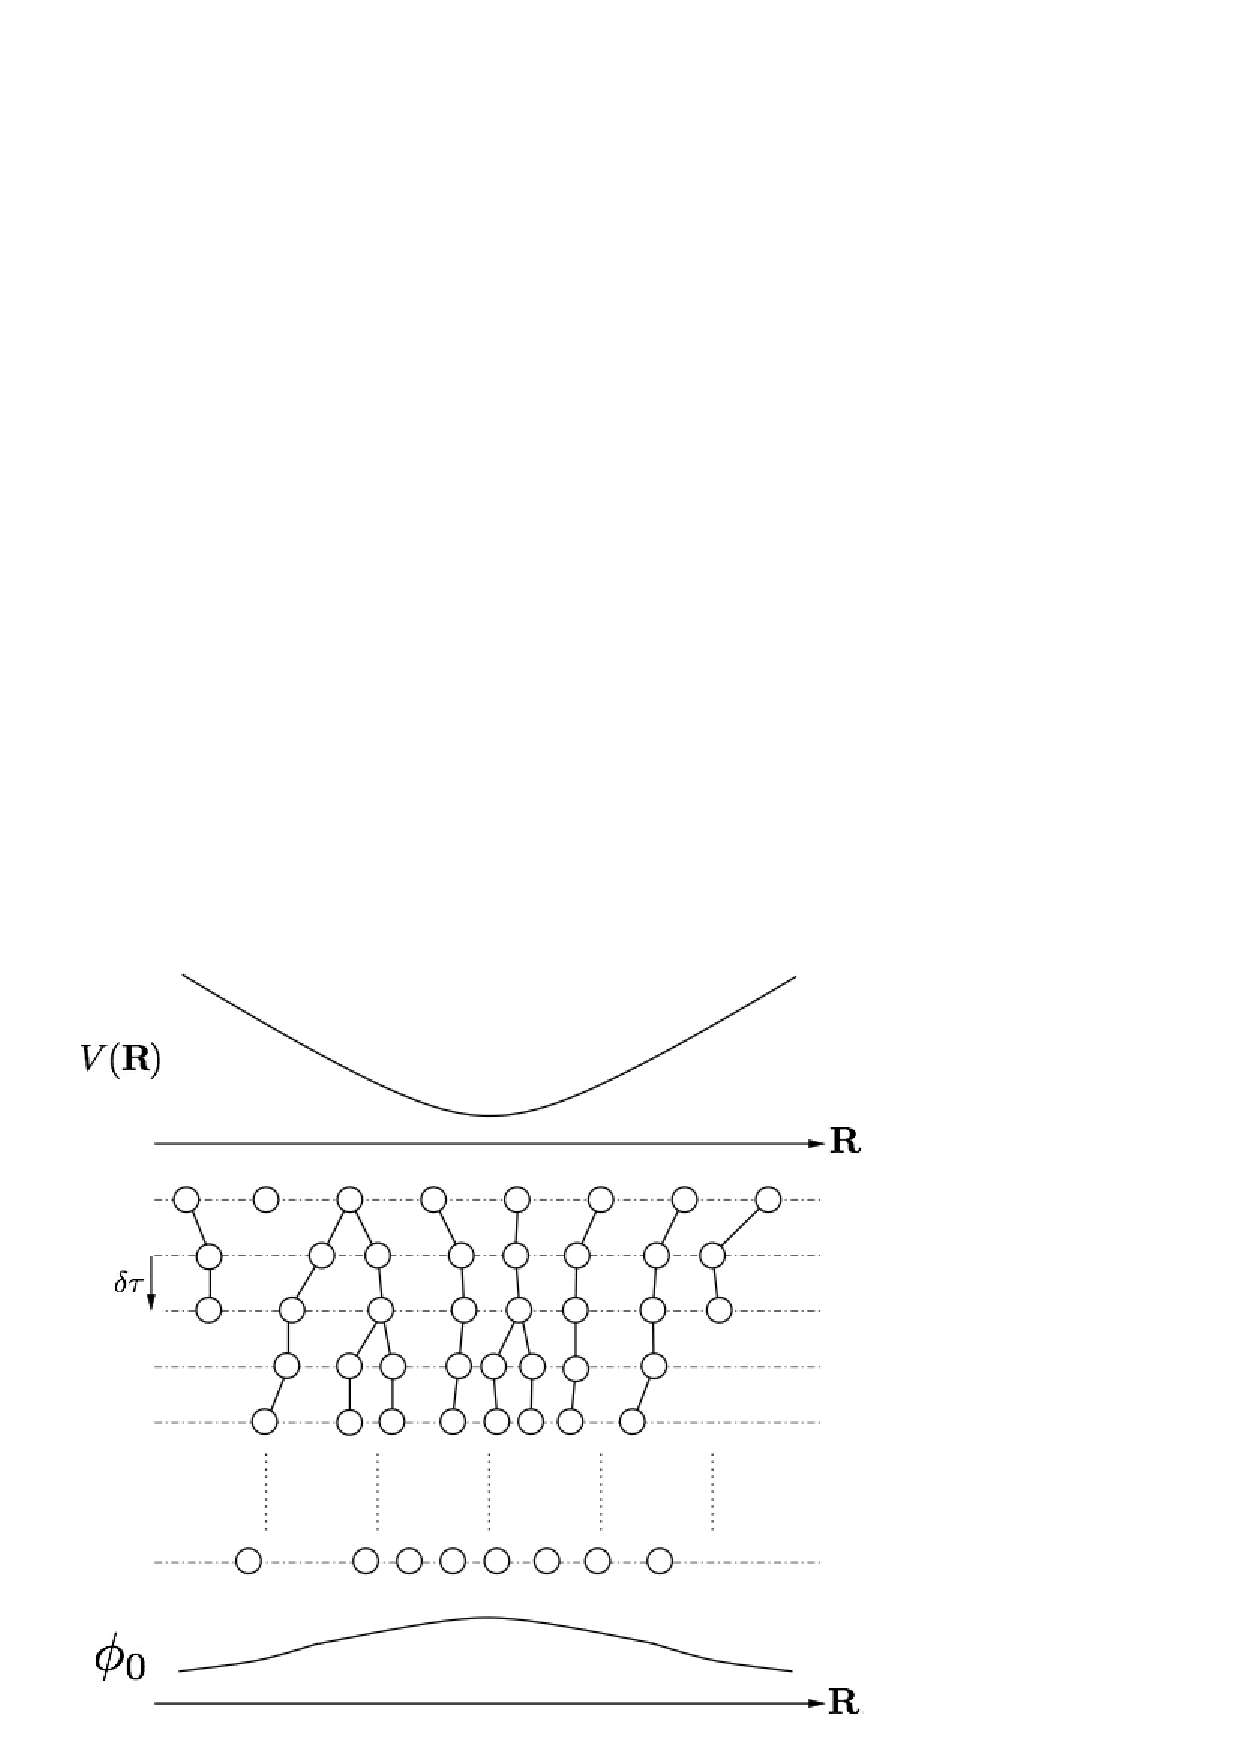
\includegraphics[width =0.49\textwidth]{DMC.pdf}
\caption[Illustration of the diffusion of walkers in DMC]{The diffusion of walkers through \textbf{R}-space. An initially even distribution of walkers is propagated through imaginary time, $\tau$. Under the influence of the potential $V(\textbf{R})$,  the distribution eventually evolves into what is representative of the ground state many-electron wave function $\psi(\textbf{R})$.}
\label{fig:DMC}
\end{center}
\end{figure}
%\begin{wrapfigure}{r}{0.3\textwidth}
%\begin{center}
%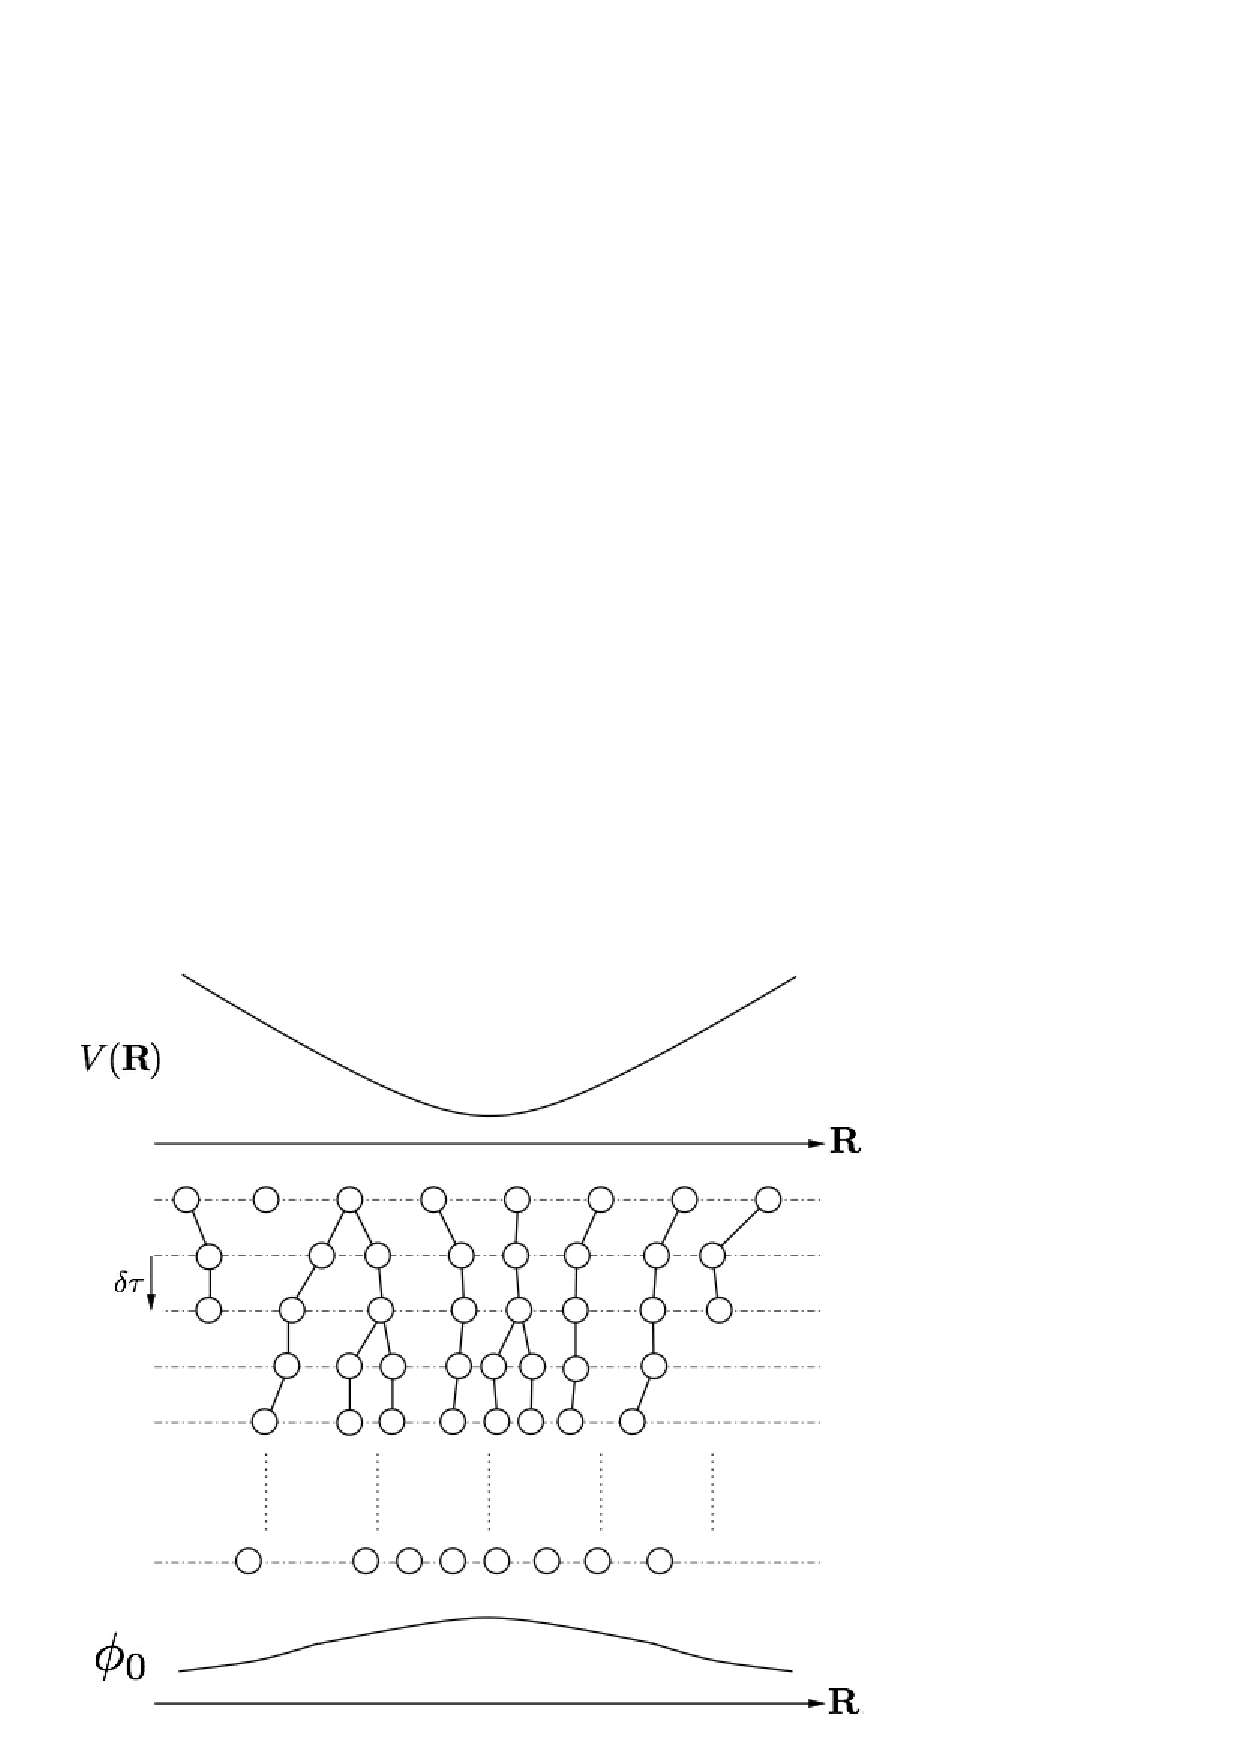
\includegraphics[width =0.3\textwidth]{DMC.pdf}
%\caption{The diffusion of walkers through \textbf{R}-space. An initial even distribution of walkers is propogated through imaginary time, $\tau$. Under the influence of the potential $V(\textbf{R})$,  The distribution eventually evolves into what is representative of the ground state many-electron wave function $\phi_0(\textbf{R})$.}
%\label{fig:Setup}
%\end{center}
%\end{wrapfigure}

It is well known that the only major obstacle preventing the exact solution of the many-electron  Schr\"{o}dinger equation via stochastic methods, such as DMC, is the fermion sign problem. This problem arises from the antisymmetry of many-electron wave functions, Eq.~\ref{eq:antiSymmetry}. As the  Schr\"{o}dinger equation becomes a diffusion equation in imaginary time, Eq.~\ref{eq:imaginaryTime}, its lowest energy solution is generally symmetric and nodeless, which directly disagrees with fermion antisymmetry. Stochastic propagation leads directly to this undesired solution in a process known as the ``boson catastrophe''\cite{Booth2009}.

One way of trying to prevent the boson catastrophe  is the fixed-node approximation\cite{Foulkes2001,BajdichMichalandMitas2009}. In this, a trial function is used to predict positive and negative regions of the wave function, thus defining a nodal surface. If a walker attempts to cross a node then it is rejected, hence constraining the propagation to disjoint areas of propagation. This procedure would be exact if the applied nodal boundaries coincided with the exact nodal hypersurface of the ground-state electronic wave function~\cite{Booth2009}. It has in fact proven very difficult to determine accurate fixed-node surfaces for large systems. 

\section*{Full Configuration-Interaction Quantum Monte Carlo}
In 2009 Booth, Alavi and Thom \cite{Booth2009} introduced a new quantum Monte Carlo method for the simulation of correlated many-electron systems in full configuration-interaction spaces. The new method is designed to simulate the many-electron imaginary-time Schr\"{o}dinger using a set of walkers that inhabit Slater determinant space, $\{D_i \}$, and evolve under the guidance of a simple set of rules; spawning, cloning, death and annihilation. The inventors of FCIQMC note three key elements of the algorithm;
\begin{enumerate}
\item As with DMC a long-time integration of the imaginary-time Schr\"{o}dinger equation is performed, however it is achieved in a space of Slater determinants
\item In a similar way to DMC the instantaneous wave function is represented by walkers instead of amplitude coefficients, allowing the description of the FCI wave function stochastically, without storing all amplitudes simultaneously
\item Walkers carry a positive or negative sign which allows for annihilation, where two walkers of opposite sign are destroyed if they coincide on the same determinant
\end{enumerate}

In order to satisfy these three key elements a long-time integration must be performed on an analogue of Eq.~\ref{eq:imaginaryTime} that is expressed in a Slater determinant basis. A set of coupled first-order differential equations for the FCI coefficients are derived\cite{Booth2009}:
\begin{equation}
\label{eq:schrodingerSlaterSpace}
-\frac{dC_i}{d\tau} = (K_{ii}-S)C_i + \sum_{j\neq i}K_{ij}C_j,
\end{equation}
where
\begin{equation}
\label{eq:KMatrixElements}
K_{ij} \equiv \Bra{D_i} K \Ket{D_j} = \Bra{D_i} H\Ket{D_j}-E_{HF}\delta_{ij},
\end{equation}
where $S$ is an adjustable energy offset\footnote{Similar to in DMC this energy offset is introduced to keep the population under control}, $C_j$ is the coefficient of the $j$th determinant in the Slater determinant expansion of the wave function (CI coefficients) and $E_{HF}$ is the Hartree-Fock energy. 

The population dynamics algorithm \cite{Booth2009,Booth2010,Booth2011} simulates the set of differential equations, Eq.~\ref{eq:schrodingerSlaterSpace}. The algorithm consists of three steps, which are performed at each time step of length $\delta\tau$:
\begin{enumerate}
\item \underline{Spawning:}  Each walker located on $D_i$ attempts to spawn another walker on a connected determinant $D_j$ with probability 
\begin{equation}
P_s(D_j\vert D_i) = \frac{\delta \tau \lvert K_{ij} \rvert}{P_{gen}(D_j\vert D_i)},
\end{equation}
where $P_{gen}(D_j\vert D_i)$ is the calculated probability of generating $D_j$\footnote{Booth \textit{et al.}\cite{Booth2009} describe how to calculate $P_{gen}$}. The sign of the spawned walker is the same as the parent if $K_{ij}<0$ and is opposite otherwise.
\item \underline{Diagonal death/cloning:} For each parent (pre-existing walker) compute
\begin{equation}
p_d(D_i) = \delta\tau(K_{ii}-S).
\end{equation}
If $p_d > 0$ the walker dies (immediately removed from simulation) with probability $p_d$ otherwise it is cloned with probability $\lvert p_d \rvert$.
\item \underline{Annihilation:} run over all remaining walkers and annihilate all opposite-sign pairs that occupy the same point in antisymmetric Slater determinant space.
\end{enumerate}
%\begin{figure}[h!]
%\begin{center}
%\includegraphics[width =0.49\textwidth]{FCIQMC.eps}
%\caption{Illustration of the spawning, cloning, death and anhilation processes as a walker %population, consisting of $+$ and $-$ signs, evolves in a Slater determinant space in imaginary %time, $\tau$. Eventually the walker population reaches a critical number and the walker growth %exhibits a characteristic plateau at which point the correlation energy can be extracted.}
%\label{fig:FCIQMC}
%\end{center}
%\end{figure}
Such an algorithm converges on the exact fermonic ground-state of the Hamiltonian in the Slater determinant basis~\cite{Booth2009}. So in this way, it prevents convergence to a bosonic solution, which is a major problem in other QMC methods. Moreover, FCIQMC simulations do not require any \emph{a priori} information and hence removes the hassle of trying to calculate a nodal structure as is inherent in DMC. 

% ------------------------------------------------------------------------

%%% Local Variables: 
%%% mode: latex
%%% TeX-master: "../thesis"
%%% End: 
